% -*- LaTeX -*- %%%%%%%%%%%%%%%%%%%%%%%%%%%%%%%%%%%%%%%%%%%%%%%%%%%%%%
%
% Template for scribing COMP163 - Computational Geometry 
%
% Spring, 2004
%
%%%%%%%%%%%%%%%%%%%%%%%%%%%%%%%%%%%%%%%%%%%%%%%%%%%%%%%%%%%%%%%%%%%%%%
%**start of header

\documentclass [12pt]{article}
\usepackage{epsfig}
\usepackage{enumitem}
\usepackage{amsmath}
\usepackage[color, leftbars]{changebar}

\usepackage{caption}
\usepackage{subcaption}


\setlength{\textwidth}{6.5in}
\setlength{\textheight}{9in}
\setlength{\oddsidemargin}{0in}
\setlength{\evensidemargin}{0in}
\setlength{\topmargin}{-0.5in}

\setlength{\parindent}{0pt}

\newtheorem{theorem}{Theorem}[section]
\newtheorem{definition}[theorem]{Definition}
\newtheorem{claim}[theorem]{Claim}
\newtheorem{lemma}[theorem]{Lemma}
\newtheorem{proof}[theorem]{Proof}

\newlength{\toppush}
\setlength{\toppush}{2\headheight}
\addtolength{\toppush}{\headsep}

\usepackage{hyperref}
\hypersetup{
    colorlinks=true,
    linkcolor=blue, % was previously black
    filecolor=magenta,
    urlcolor=blue,
    pdftitle={Template}
}
\urlstyle{same}

%\doheading{2}{title}{Last Revised: January, 2004}
%\htitle{title}

\def\subjnum{Comp 163}
\def\subjname{Computational Geometry}

\def\doheading#1#2#3{\vfill\eject\vspace*{-\toppush}%
  \vbox{\hbox to\textwidth{{\bf} \subjnum: \subjname \hfil Amy Bui}%
    \hbox to\textwidth{{\bf} Tufts University, Fall 2022 \hfil#3\strut}%
    \hrule}}

\newcommand{\htitle}[1]{\vspace*{3.25ex plus 1ex minus .2ex}%
\begin{center}
{\large\bf #1}
\end{center}} 

%%%%%%%%%%%%%%%%%%%%%%%%%%%%%%%%%%%%%%%%%%%%%%%%%%%%%%%%%%%%%%%%%%%

\begin{document}
\doheading{2}{title}{HW 1}
% \htitle{Homework 1}
% \bigskip 
% \bigskip 
%%%%%%%%%% begin text after this line %%%%%%%%%%%%%%

    %%%%%%%%%%%%%%%%%%%%%%%%%%%%%%%%%%%%%%%%%%%%%%%%%%%%%%%%%%%%%%%%%%%%%%%%%
    \section{Left Turn and Convexity}
    \label{sec:one}

        \begin{enumerate}[label=(\alph*)]
            \item 
            Derive and verify that, for the given points $A = (x_a, y_a)$, $B = (x_b, y_b)$, and $C = (x_c, y_c)$ (in this order), the sign of the determinant is positive if $A$, $B$, and $C$ appear in counterclockwise (ccw). The determinant can be calculated by:
            % $$
            % D = \begin{vmatrix}
            %     x_a & y_a & 1 \\
            %     x_b & y_b & 1 \\
            %     x_c & y_c & 1 
            %     \end{vmatrix} , 
            % $$
            % $A$, $B$, and $C$ appear in counterclockwise (ccw) order on the boundary of $\Delta ABC$ if and only if $D$ is positive (i.e. $A$, $B$, $C$ form a left turn if $D > 0$).
            \begin{align*}
                D &= \begin{vmatrix}
                        x_a & y_a & 1 \\
                        x_b & y_b & 1 \\
                        x_c & y_c & 1 
                        \end{vmatrix} 
                = x_a \begin{vmatrix}
                    y_b & 1 \\
                    y_c & 1 
                \end{vmatrix} 
                - y_a \begin{vmatrix}
                    x_b & 1 \\
                    x_c & 1 
                \end{vmatrix} 
                + 1 \begin{vmatrix}
                    x_b & y_b \\
                    x_c & y_c
                \end{vmatrix} \\
                % &= x_a (y_b - y_c) - y_a (x_b - x_c) + (x_b y_c - y_b x_c) \\
                &= (x_a y_b - x_a y_c) + (x_c y_a - x_b y_a) + (x_b y_c - x_c y_b)
            \end{align*}

            % \textbf{\textsc{Linear Algebra}}

            Notice the result is the cross product of the two vectors $\overrightarrow{AB} = \langle x_b - x_a, y_b - y_a, 0 \rangle$ and $\overrightarrow{BC} = \langle x_c - x_b, y_c - y_b, 0 \rangle$, i.e. $\overrightarrow{AB} \times \overrightarrow{BC}$:
            \begin{align*}
                % \overrightarrow{AB} = \langle x_b - x_a, y_b - y_a, 0 \rangle \\ 
                % \overrightarrow{BC} = \langle x_c - x_b, y_c - y_b, 0 \rangle \\ 
                \overrightarrow{AB} \times \overrightarrow{BC} &= 
                \begin{vmatrix}
                    i & j & k \\
                    x_b - x_a & y_b - y_a & 0 \\ 
                    x_c - x_b & y_c - y_b & 0
                \end{vmatrix} \\
                % &= \big[(x_b - x_a)(y_c - y_b) - (y_b - y_a)(x_c - x_b)\big] k \\ 
                &= \big[(x_a y_b - x_a y_c) + (x_c y_a - x_b y_a) + (x_b y_c - x_c y_b)\big] k
            \end{align*}

            By the right-hand rule convention, when the cross product is positive, the direction along the path from $A \rightarrow B \rightarrow C \rightarrow A$ of the boundary of $\Delta ABC$ is ccw, where our $C$ is to the ``left'' of directed line $\overrightarrow{AB}$, because the direction of the vector perpendicular to the two vectors is in the positive direction (Fig. \ref{fig:ccwtriangle}); when the cross product is negative, the direction along the path from $A \rightarrow B \rightarrow C \rightarrow A$ of the boundary of $\Delta ABC$ is clockwise, because the direction of the vector perpendicular to the two vectors is in the negative direction (Fig. \ref{fig:cwtriangle}). Therefore, the sign of the determinant can tell us when three points are given in ccw or cw order.

            Reference: \cite{crossprod2vec} \cite{mathcurvorien}

            \begin{figure}[h]
                \begin{tabular}{cc}
                    \begin{subfigure}{0.5\textwidth}
                        \centering 
                        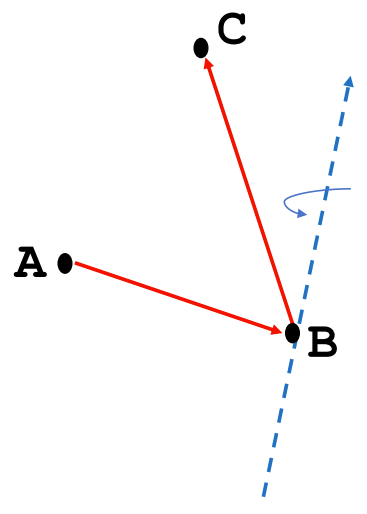
\includegraphics[width=0.4\textwidth]{images/ccwRightHand.PNG}
                        \caption{Positive cross product}
                        \label{fig:ccwtriangle}
                    \end{subfigure}
                    & 
                    \begin{subfigure}{0.5\textwidth}
                        \centering 
                        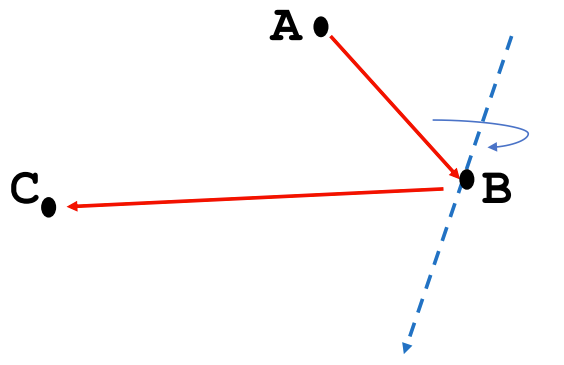
\includegraphics[width=.7\textwidth]{images/cwRightHand.PNG}
                        \caption{negative cross product}
                        \label{fig:cwtriangle}
                    \end{subfigure} 
                \end{tabular}
                \caption{Visualization of $\protect\overrightarrow{AB} \times \protect\overrightarrow{BC}$}
                \label{fig:1a}
            \end{figure}

            \pagebreak
            % \textbf{\textsc{Geometry}}
            % \begin{figure}[h]
            %     \begin{tabular}{cc}
            %         \begin{subfigure}{0.5\textwidth}
            %             \centering 
            %             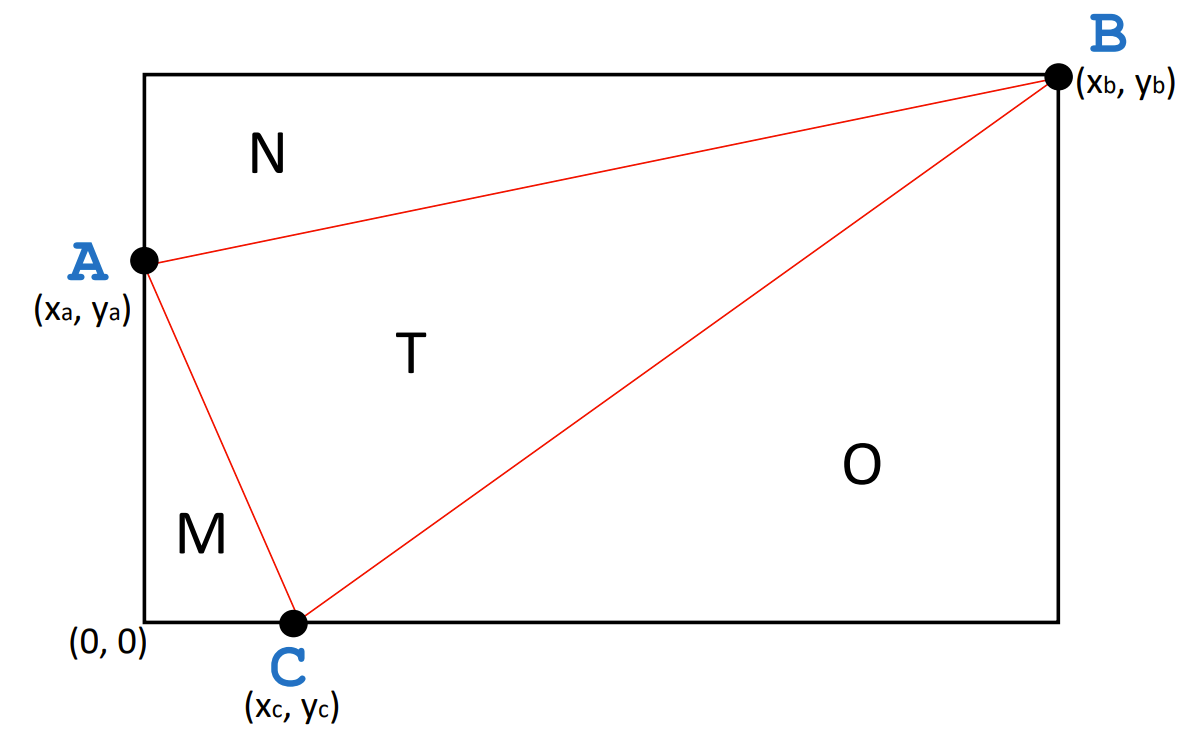
\includegraphics[width=1\textwidth]{images/cwtriangle.PNG}
            %             \caption{}
            %             \label{cwtriangle}
            %         \end{subfigure} & 
            %         \begin{subfigure}{0.5\textwidth}
            %             \centering 
            %             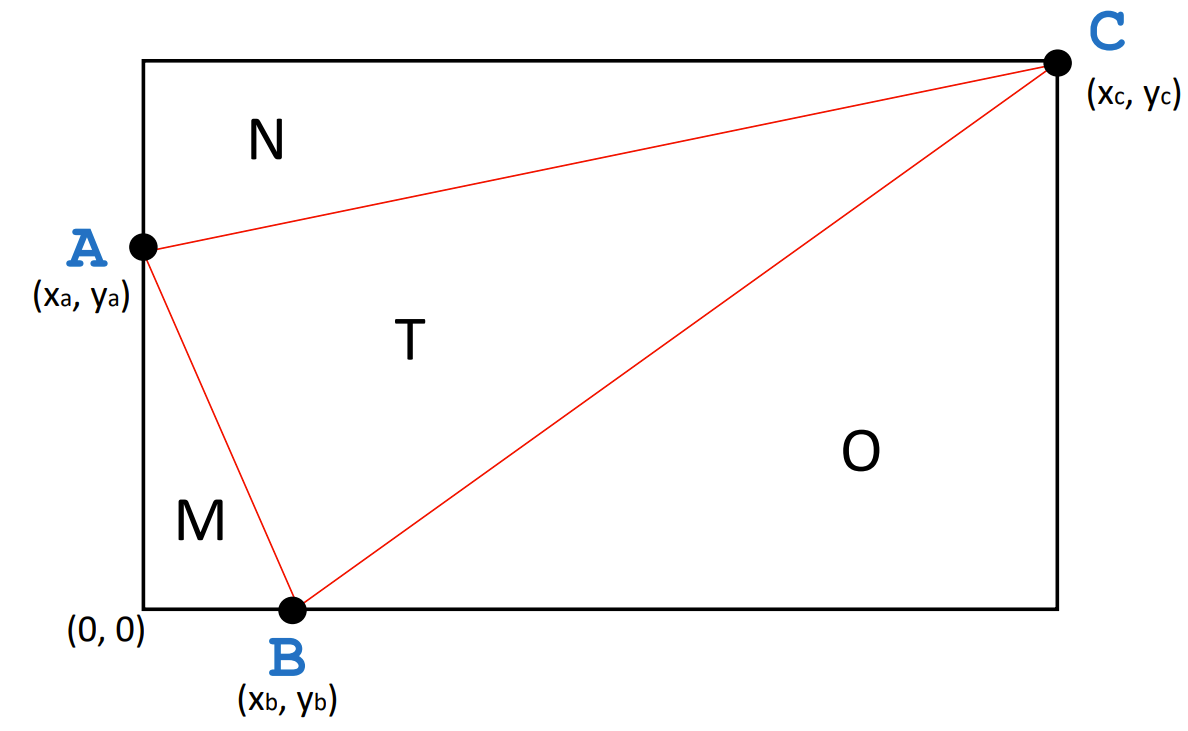
\includegraphics[width=1\textwidth]{images/ccwtriangle.PNG}
            %             \caption{}
            %             \label{ccwtriangle}
            %         \end{subfigure}
            %     \end{tabular}
            % \end{figure}


            % Reference: \cite{officehours}

            \item Describe an algorithm to test if polygon $P$ (given by a circularly linked list of its $n$ vertices in order) is convex. 
            
            From class, a convex polygon is such that, walking along the boundary of the polygon, all angles ``turn'' in the same ``direction'', resulting in all internal angles being less than $180^\circ$ and only consecutive segments intersecting.
            
            *Let there exist a method that outputs the sign of the determinant of three given coordinate points, and call it \textsc{DeterminantSign}. Assume it runs $O(1)$ time by plugging in the coordinate values in the formula(s) like those mentioned in part (a).
             
            \emph{\textbf{Input}}: A circularly linked list of the $n$ ordered vertices of polygon $P$. We will call these vertices in their sequence $p_1, p_2, ..., p_n$, where $p_1$ is arbitrarily selected as the ``first'' vertex we examine in the algorithm below, $p_2$ is the ``next'' node/vertex of $p_1$, etc.

            \emph{\textbf{Output}}: \textbf{true} or \textbf{false} if $P$ is convex.

            \cbcolor{blue}
            \textsc{isConvex($P$)}:
            \cbstart
            \begin{enumerate}[label=\arabic*.]
                \item $A \leftarrow p_1$; $B \leftarrow p_2$; $C \leftarrow p_3$ \hspace{1cm} $\Theta(1)$
                \item \texttt{direction} $\leftarrow$ \textsc{DeterminantSign}($A, B, C$) \hspace{1cm} $\Theta(1)$
                \item \textbf{for} $i \leftarrow 2$ \textbf{to} $n$ \hspace{1cm} $\Theta(n)$
                \item \hspace{1cm} $A \leftarrow B$; $B \leftarrow C$; $C \leftarrow C$.\textsf{next} \hspace{1cm} $\Theta(1)$
                \item \hspace{1cm} \texttt{turn} $\leftarrow$ \textsc{DeterminantSign}($A, B, C$) \hspace{1cm} $\Theta(1)$
                \item \hspace{1cm} \textbf{if} \texttt{turn} $\neq$ \texttt{direction} \textbf{then} return \textbf{false}
                \item return \textbf{true}
            \end{enumerate}
            \cbend

            \begin{description}
                \item[Correctness]: The algorithm examines each adjacent angle of the polygon formed by three adjacent points. The direction (in terms of left/right or positive/negative) of the first arbitrary (interior) angle chosen is given by \textsf{direction} (line 2) and formed from 3 vertices. I show by induction that this algorithm works for all polygons of $k \leq n$ vertices, where $3 \leq k \leq n$.
                
                For $k = 3$ vertices (triangle), it is trivially true that $P$ is a convex polygon, and the  direction of the $k$ angles match and all are acute. For $k = \{3, ..., i\}$, let all the directions of the angles up to the angle about $p_{i-1}$ (i.e. $\angle p_{i-2}, p_{i-1}, p_i$) match the first, thus far, and therefore $\{p_1 ... p_i\}$ is convex. The next angle formed with the $i\rightarrow\textsf{next}^{th}$ vertex, given by $\angle p_{i-1}, p_{i}, p_{i\rightarrow\textsf{next}}$, will have a \textsf{turn} that either does or doesn't match \textsf{direction}. If it matches, $P$ is convex because all turns are the same. If it doesn't, $P$ is not convex because the angle makes it either a concave polygon or complex polygon.
                

                \item[Complexity]: Let accessing the next adjacent node in the linked list be a $O(1)$ time operation. Each line in the algorithm runs $O(1)$ time except for the for loop in lines 3 - 6. The for loop examines the ``turn'' of only each adjacent triple on the list of vertices. Therefore, the for loop runs $O(n)$ time. We are not concerned with any sorting of the vertices here. Therefore, the total runtime of the algorithm is $O(n)$.
            \end{description}

        \end{enumerate}

    \pagebreak
    % END %%%%%%%%%%%%%%%%%%%%%%%%%%%%%%%%%%%%%%%%%%%%%%%%%%%%%%%%%%%%%%%%%%%



    %%%%%%%%%%%%%%%%%%%%%%%%%%%%%%%%%%%%%%%%%%%%%%%%%%%%%%%%%%%%%%%%%%%%%%%%%
    \section{Unordered Divide-and-Conquer Convex Hull}
    \label{sec:two}

    \begin{enumerate}[label=(\alph*)]
        \item For $P_1$ and $P_2$ to share a support line, the line must have at least one vertex from each polygon on it, and all the vertices of both polygons must be to one side of the line. If $P_1$ and $P_2$ share no vertices, then they are either 1) completely disjointed, 2) one is completely interior to the other, or 3) their edges intersect. 
        
        If they are \textbf{disjointed}, then $P_1$ and $P_2$ can only have 2 support lines in common, both of which would create the new edges of the convex hull created from $P_1 \cup P_2$, regardless of the values of $n_1$ and $n_2$. In other words, each vertex of $P_1$ has 1 or 0 shared support line with $P_2$. (Fig. \ref{fig:supportline1a})
            \begin{figure}[h]
                \centering 
                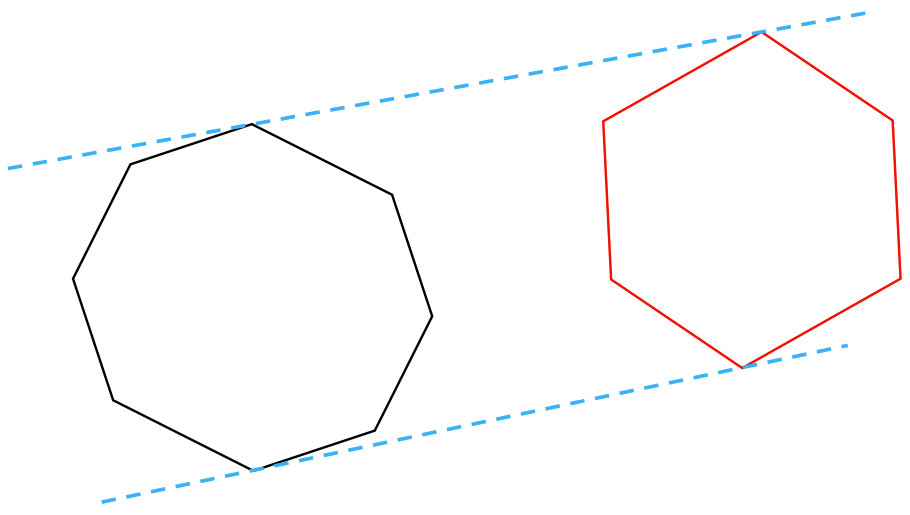
\includegraphics[width=0.4\textwidth]{images/supportline1a.PNG}
                \caption{Shared support lines (blue) of two disjointed polygons.}
                \label{fig:supportline1a}
            \end{figure}
        
        If one is \textbf{interior} to the other, regardless of the values of $n_1$ and $n_2$, then there are 0 support lines, because any support lines the interior polygon has would intersect the exterior polygon, and any support lines the exterior polygon has would never share a vertex from the interior polygon. (Fig. \ref{fig:supportline2a})
            \begin{figure}[h]
                \centering 
                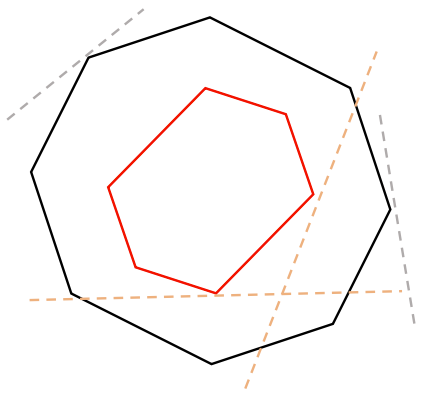
\includegraphics[width=0.2\linewidth]{images/supportline2a.PNG}
                \caption{Two polygons with no shared support lines. The exterior polygon's support lines (grey) never touch the interior polygon, and the interior polygon's support lines (orange) bisects the exterior polygon.}
                \label{fig:supportline2a}
            \end{figure}
        
            \pagebreak

        Finally, the most number of support lines that can occurr at one vertex is 2, because that is the number of edges a vertex has that could intersect the other polygon. It may have 0 shared support lines in the case that one vertex of $P_1$ is interior to $P_2$; it may have 1 shared support line in the case that only one of the edges formed intersects the other polygon, then one of the points of that edge will share a support line with one of the points in the other polygon (Fig. \ref{fig:supportline3a} - \ref{fig:supportline3g}). Or it can have 2 shared support lines when both edges of the vertex intersects edges of the other polygon (Fig. \ref{fig:supportline3b} and \ref{fig:supportline3g}). This can happen at most $2 \times \texttt{min}(n_1, n_2)$, limited by the number of vertices of the lesser polygon and depending on how the two polygons overlap.


        % Finally, the most number of support lines that can occurr at one vertex is 2, because that is when the vertex of one convex polygon is in a position ``between'' two vertices of the other polygon, and the edges of the polygon that include that 1 vertex intersects the greater polygon at the edges formed by those two vertices (Fig. \ref{fig:supportline3b}); otherwise,  This can happen at most $2 \times \texttt{min}(n_1, n_2)$, limited by the number of vertices of the lesser polygon and depending on how the two polygons overlap.

        % There can be 0 common support lines wherever $P_1$ and $P_2$ share an edge, because that would place the vertices of the polygons on opposite sides of the line. Figure ...
        
        Therefore, the number of common support lines of $P_1$ and $P_2$ is at most $2 \times \texttt{min}(n_1, n_2)$.

        \begin{figure}[h]
            \begin{tabular}{ccc}
                \begin{subfigure}{0.33\textwidth}
                    \centering
                    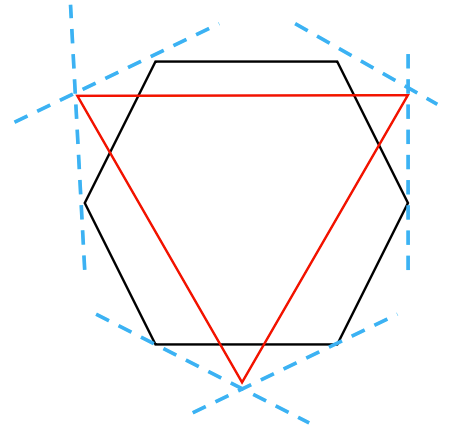
\includegraphics[width=0.7\textwidth]{images/supportline3b.PNG}
                    \caption{}
                    \label{fig:supportline3b}
                \end{subfigure} &
                \begin{subfigure}{0.33\textwidth}
                    \centering
                    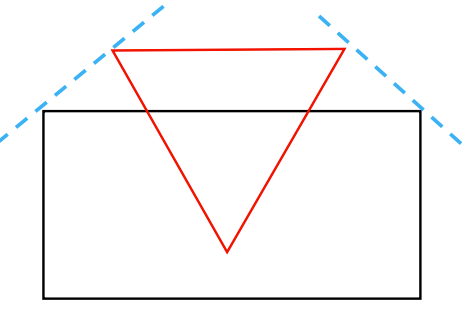
\includegraphics[width=0.7\textwidth]{images/supportline3a.PNG}
                    \caption{}
                    \label{fig:supportline3a}
                \end{subfigure} & 
                \begin{subfigure}{0.33\textwidth}
                    \centering
                    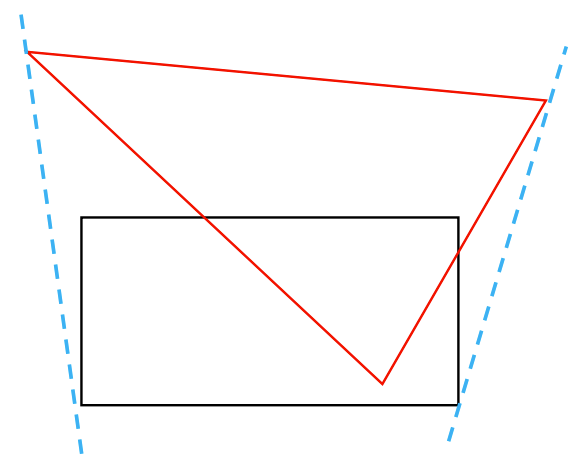
\includegraphics[width=0.7\textwidth]{images/supportline3c.PNG}
                    \caption{}
                    \label{fig:supportline3c}
                \end{subfigure}\\
                \begin{subfigure}{0.33\textwidth}
                    \centering
                    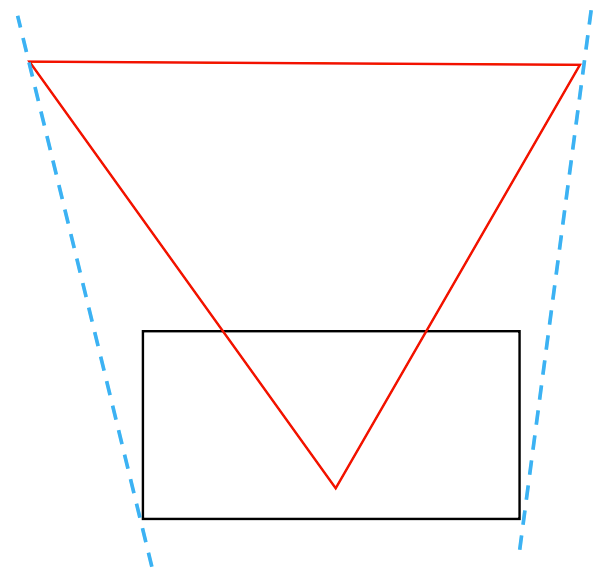
\includegraphics[width=0.7\textwidth]{images/supportline3d.PNG}
                    \caption{}
                    \label{fig:supportline3d}
                \end{subfigure} & 
                \begin{subfigure}{0.33\textwidth}
                    \centering
                    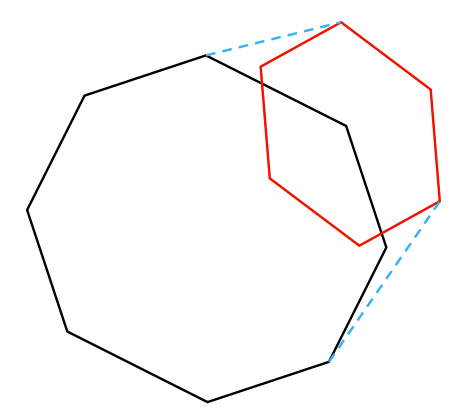
\includegraphics[width=0.7\textwidth]{images/supportline3e.PNG}
                    \caption{}
                    \label{fig:supportline3e}
                \end{subfigure} &
                \begin{subfigure}{0.33\textwidth}
                    \centering
                    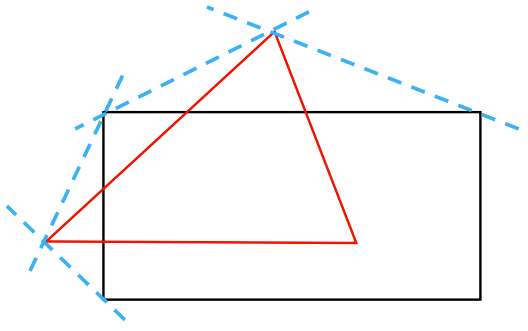
\includegraphics[width=0.7\textwidth]{images/supportline3g.PNG}
                    \caption{}
                    \label{fig:supportline3g}
                \end{subfigure}
            \end{tabular}
            \caption{Possible shared support lines (blue) formed in various ways two polygons overlap. The red polygon indicates it has fewer or equal number of vertices than the black polygon.}
            \label{fig:overlappingpolygons}
        \end{figure}

        Reference: \cite{officehours}
 
        \pagebreak
        \item I specify an algorithm that computes the convex hull of convex polygons $P \cup Q$. Since they are already known to be convex, their vertices are already sorted.
        

        \emph{\textbf{Input}}: The sorted vertices of convex polygons $P$ and $Q$, ordered respectively by $\{ p_1, ..., p_{n}\}$ and $\{ q_1, ..., q_{m}\}$. Note that $|P| = n$ and $|Q| = m$, and let $N = n + m$.

        \emph{\textbf{Output}}: $\mathcal{CH}(P \cup Q)$

        
        \cbcolor{blue}
            \cbstart
            \textsc{MergeConvexHulls($P$, $Q$)}:
            \begin{enumerate}[label=\arabic*.]
                \item $X \leftarrow$ \emph{Merge} $P$ and $Q$. \hspace{1cm} $\Theta(N)$
                \item Find the convex hull of sorted $X$ using any convex hull finding algorithm on a presorted list. I suggest \textsc{GrahamScan}. 
                
                So $Y \leftarrow$ \textsc{GrahamScan}$(X)$ \hspace{1cm} $\Theta(N)$

                \item return $Y$
            \end{enumerate}
        \cbend


        The runtime is $O(N)$ because it takes $O(N)$ time to sort the already sorted elements of $P$ and $Q$ into one list $X$. And then we are running Graham Scan on a presorted list, which itself is then $O(N)$ time.
        
        \item I specify a divide-and-conquer algorithm that uses \textsc{MergeConvexHulls} without presorting to find the convex hull of an arbitrary set of $n$ points in set $S$.
        
        \cbcolor{blue}
            \cbstart
            \textsc{DC-ConvexHull($S$)}:
            \begin{enumerate}[label=\arabic*.]
                \item $m \leftarrow \frac{n}{2}$
                \item $L \leftarrow S[0:m-1]$ and $R \leftarrow S[m:n-1]$
                \item $L' \leftarrow$ \textsc{DC-ConvexHull($L$)}
                \item $R' \leftarrow$ \textsc{DC-ConvexHull($R$)}
                \item $S' \leftarrow$ \textsc{MergeConvexHulls($L'$, $R'$)} \hspace{1cm} $\Theta(n)$
                \item return $S'$
            \end{enumerate}
        \cbend

        The runtime is $O(n \log n)$ because it divides $S$ in half to find the convex hulls of the separated set by making recursive call to the divide-amd-conquer algorithm, and takes linear time to ``merge'' the two convex hulls/polygons that were found, which results in the convex hull formed by the two convex polygons.

    \end{enumerate}


    \pagebreak
    % END %%%%%%%%%%%%%%%%%%%%%%%%%%%%%%%%%%%%%%%%%%%%%%%%%%%%%%%%%%%%%%%%%%%


    %%%%%%%%%%%%%%%%%%%%%%%%%%%%%%%%%%%%%%%%%%%%%%%%%%%%%%%%%%%%%%%%%%%%%%%%%
    \section{Three}
    \label{sec:three}

    Given a set $S$ of $n$ planar points in general position and in arbitrary order, I construct these polygons with the following algorithms. Any figure is meant to be on xy-plane.

    \begin{enumerate}[label=(\alph*)]
        \item A simple monotone polygon $R$ whose vertices are exactly the vertices of $S$, which contains the line segment given by the min and max x-coord vertices of $S$. 

        \cbcolor{blue}
            \cbstart
            \textsc{MonotoneHull($S$)}:
            \begin{enumerate}[label=\arabic*.]
                \item $S' \leftarrow$ sort $S$ by x-coordinate. $\Theta(n\log n)$
                \item Create the line segment ($y = mx + b$) from the first and last vertices in $S'$ (min and max x-coord vertics of $S$). Let $b$ be this line's y-intersection, and $m$ the slope.
                \item \textbf{for} $i \leftarrow 0$ to $n$ \hspace{1cm}$\Theta(n)$
                \item \hspace{1cm} $B[i] \leftarrow y_{S'[i]} - m x_{S'[i]}$ 
                 
                    \hspace{1cm} (\emph{the y-insersection of the line given by} 
                
                    \hspace{1cm} \emph{the point $S'[i]$ and the slope $m$})
                \item $j \leftarrow 1$, $R[0] \leftarrow S'[0]$
                \item \textbf{for} $i \leftarrow 1$ to $n$ \hspace{1cm}$\Theta(n)$
                \item \hspace{1cm} \textbf{if} $B[i] \geq b$ 
                \item \hspace{1.5cm} \textbf{then} $R[j] \leftarrow S'[i]$, $j\leftarrow j + 1$
                \item \textbf{for} $i \leftarrow n - 1$ downto $0$ \hspace{1cm}$\Theta(n)$
                \item \hspace{1cm} \textbf{if} $B[i] < b$ 
                \item \hspace{1.5cm} \textbf{then} $R[j] \leftarrow S'[i]$, $j\leftarrow j + 1$
                \item return $R$
            \end{enumerate}
        \cbend

        This algorithm runs $\Theta(n\log n)$ time due to soring the points by the x-coordinates (line 1). We can find, in constant time, the slope and y-intersection of the line segment \textbf{L} given by the min and max x-coord points in $S'$ (line 2, Fig. \ref{fig:mono1}). Using that $m$ and $b$, we can create a list of the y-intercepts of each point in $S'$ on a line of slope $m$, which is linear time. This tells us whether or not a point in $S$ is above or below the main line segment (Fig. \ref{fig:mono2}). Finally, we compute $R$ by finding the list of points above the line segment in order of the sorted $S'$ (loop 6), and adding to it the points below the line segment (found the same way in reverse order and discarding any duplicate end points) (loop 9, Fig. \ref{fig:mono2}), this runs in linear time. (Alternatively, if for each point we found above \textbf{L} were removed from $S'$, we can simply reverse and append the remaining $S'$ to $R$). The resulting polygon is monotone with respects to our line segment \textbf{L}, because all lines perpendicular to \textbf{L} intersects $R$ at most twice (Fig. \ref{fig:mono3}).
    \end{enumerate}
        \pagebreak

        \begin{figure}[h] 
            \centering
            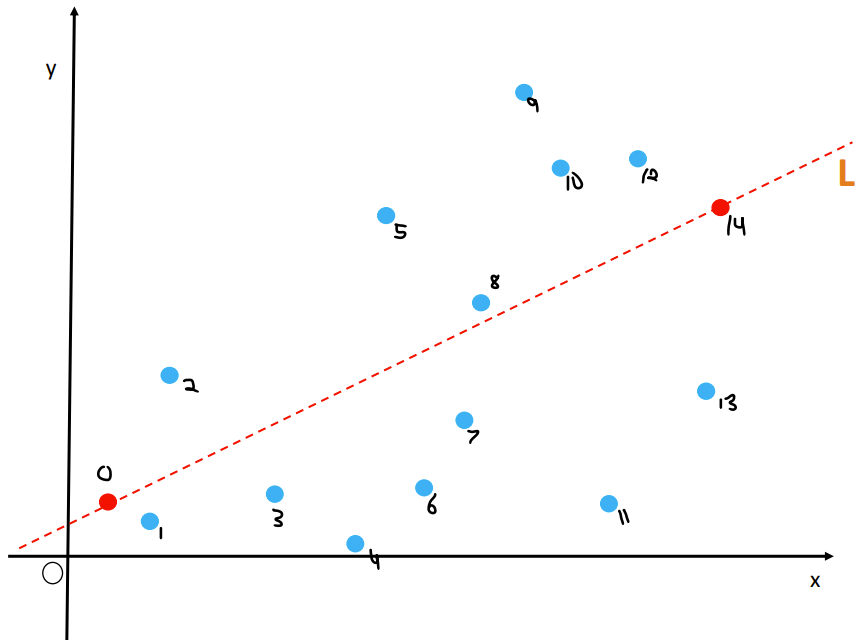
\includegraphics[width=0.55\textwidth]{images/monotonehull1.PNG}
            \caption{Set $S$ of $n$ points, labeled in order sorted by their x-coordinates. Line \textbf{L} is given by the min and max x-coordinate points in $S$.}
            \label{fig:mono1}
        \end{figure}

        \begin{figure}[h] 
            \centering
            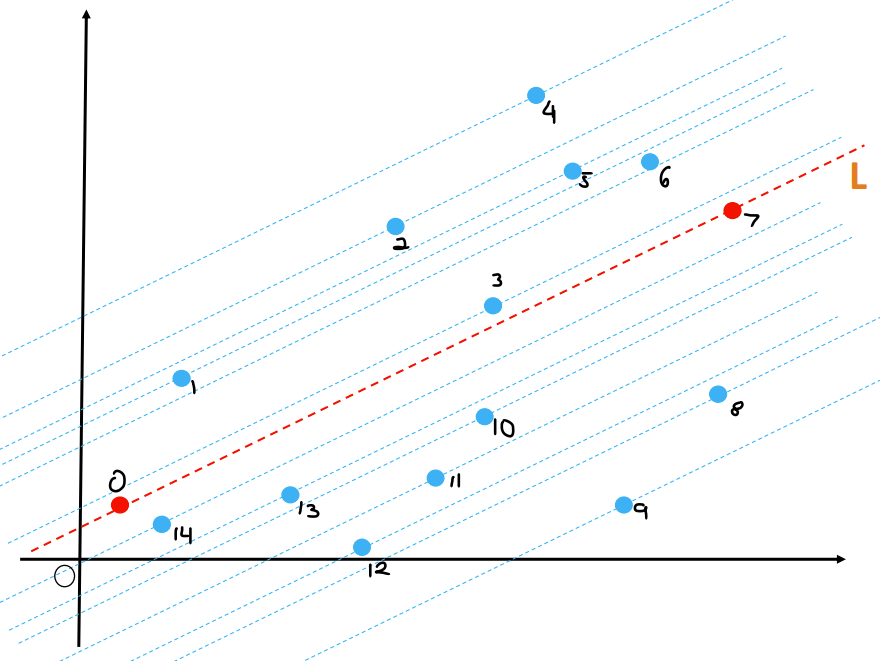
\includegraphics[width=0.55\textwidth]{images/monotonehull2.PNG}
            \caption{Every point in $S$ on a line with slope $m$ is sorted by their y-intercepts above \textbf{L} (ascending x-coord order) and below \textbf{L} (descending x-coord order).}
            \label{fig:mono2}
        \end{figure}
        \pagebreak

        \begin{figure}[h] 
            \centering
            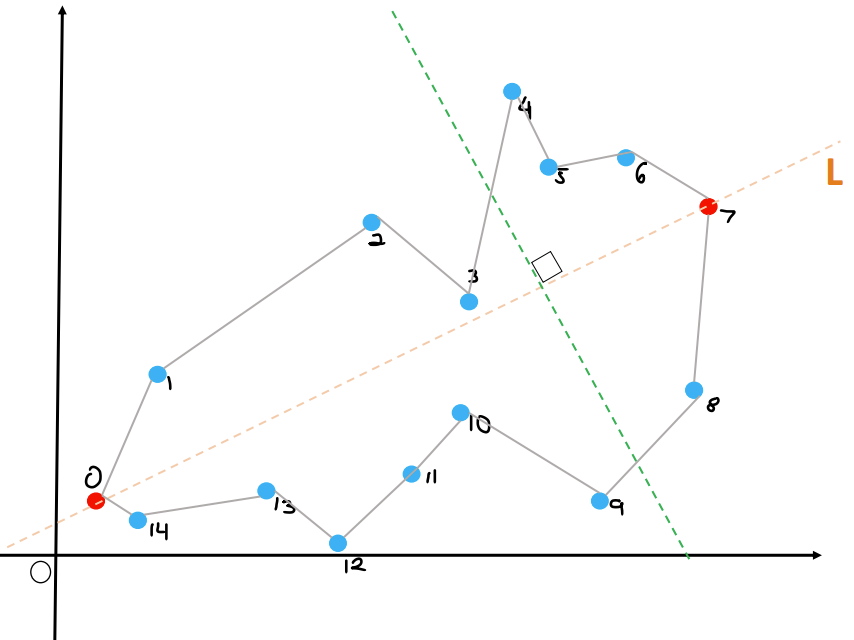
\includegraphics[width=0.6\textwidth]{images/monotonehull3.PNG}
            \caption{Resulting monotone polygon $R$ from set $S$. Every line orthongonal to \textbf{L}, such as the green line, intersects the polygon at most twice.}
            \label{fig:mono3}
        \end{figure}

        % \begin{figure}[h] 
        %     \begin{tabular}{c}
        %         \begin{subfigure}{0.8\textwidth}
        %             \centering
        %             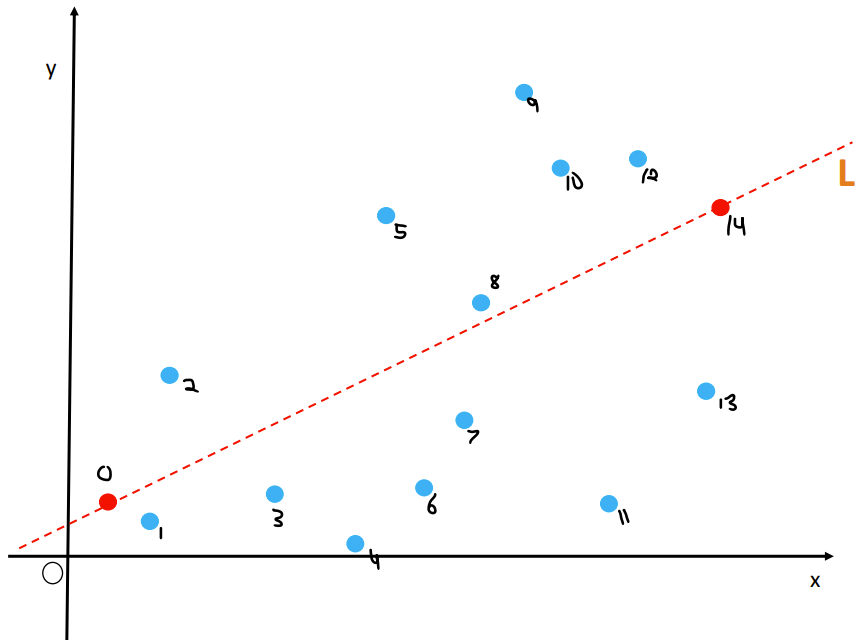
\includegraphics[width=0.6\textwidth]{images/monotonehull1.PNG}
        %             \caption{}
        %             \label{fig:mono1}
        %         \end{subfigure} \\
        %         \begin{subfigure}{0.8\textwidth}
        %             \centering
        %             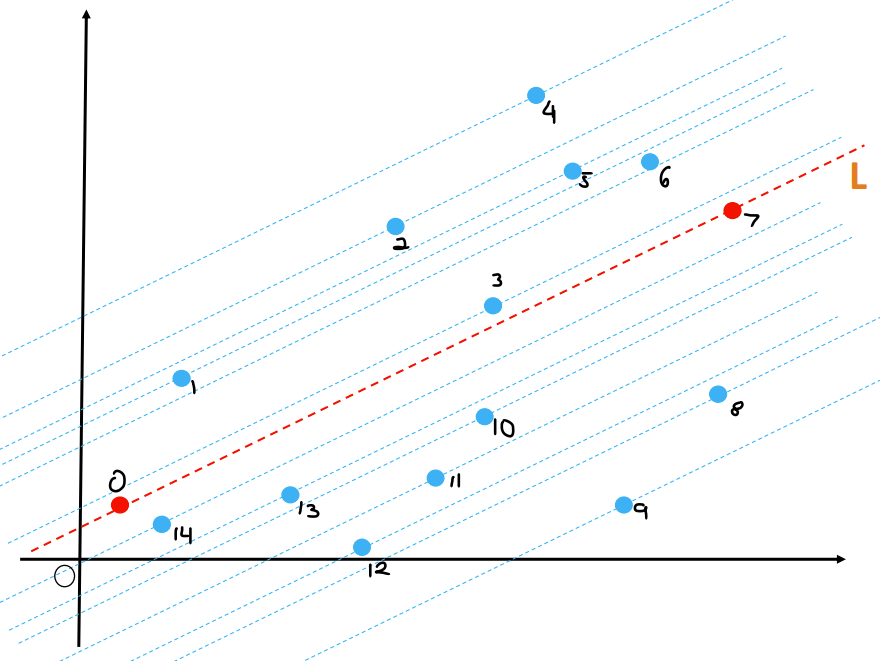
\includegraphics[width=0.6\textwidth]{images/monotonehull2.PNG}
        %             \caption{}
        %             \label{fig:mono2}
        %         \end{subfigure}\\
        %         \begin{subfigure}{0.8\textwidth}
        %             \centering
        %             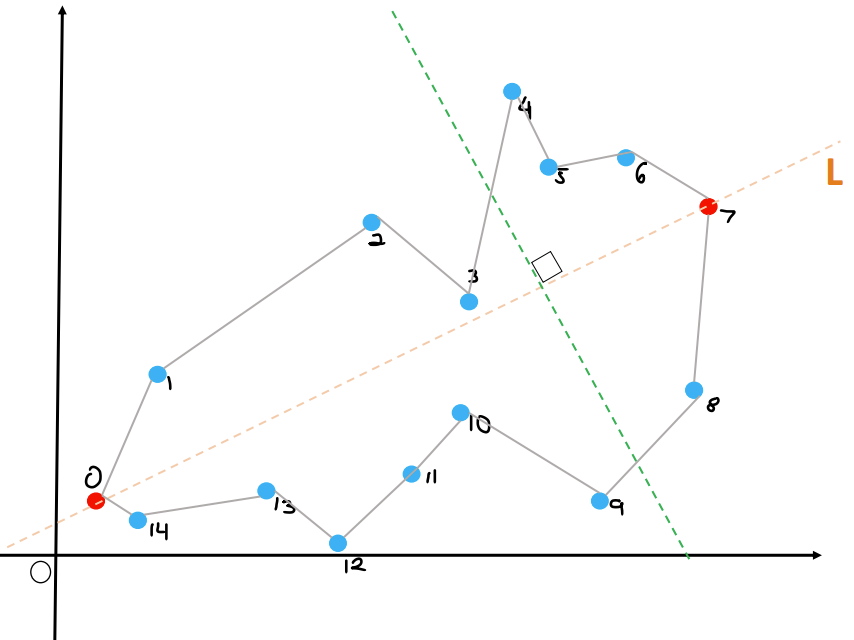
\includegraphics[width=0.6\textwidth]{images/monotonehull3.PNG}
        %             \caption{}
        %             \label{fig:mono3}
        %         \end{subfigure} \\
        %     \end{tabular}
        % \end{figure}

        \pagebreak

        \begin{enumerate}[label=(\alph*)]
            \setcounter{enumi}{1}

        \item A simple starshaped polygon $P$ whose vertices are exactly the points in S for which the min x-coord point in $S$ ``sees'' every point in $P$.
        
        \cbcolor{blue}
            \cbstart
            \textsc{StarHull($S$)}:
            \begin{enumerate}[label=\arabic*.]
                \item $p_0 \leftarrow $ smallest x-coordinate point in $S$. \hspace{1cm}$\Theta(n)$
                \item \textbf{for} $i \leftarrow 0$ to $n-1$    \hspace{1cm}$\Theta(n)$
                \item \hspace{1cm} $p_i \leftarrow S[i]$
                \item \hspace{1cm} \textbf{if} $p_i = p_0$ 
                \item \hspace{1.5cm} \textbf{then} $M[i] \leftarrow \infty$
                \item \hspace{1.5cm} \textbf{else} $M[i] \leftarrow$ slope $m$ of line $\overline{p_0 p_i}$, \hspace{1cm} $m = \frac{y_i - y_0}{x_i - x_0}$
                \item $P \leftarrow $ sort $S$ by their slope values in $M$ (decending). \hspace{1cm} $\Theta(n \log n)$
                \item return $P$ 
            \end{enumerate}
        \cbend

        This algorithm runs $\Theta(n \log n)$ time due to sorting the points in $S$ by their assigned slopes with regards to $p_0$ in $M$ (line 7). Sorting the points by their slopes ensures that the smallest x-coordinate point in $S$ ``sees'' every point in the resulting starshaped polygon $P$, because every line segment created by $p_0$ and a point in $P$ would not intersect another edge (Fig. \ref{fig:bigstar}). I prove this by induction on the size of $S$.

        % \begin{figure}[h] 
        %     \centering
        %     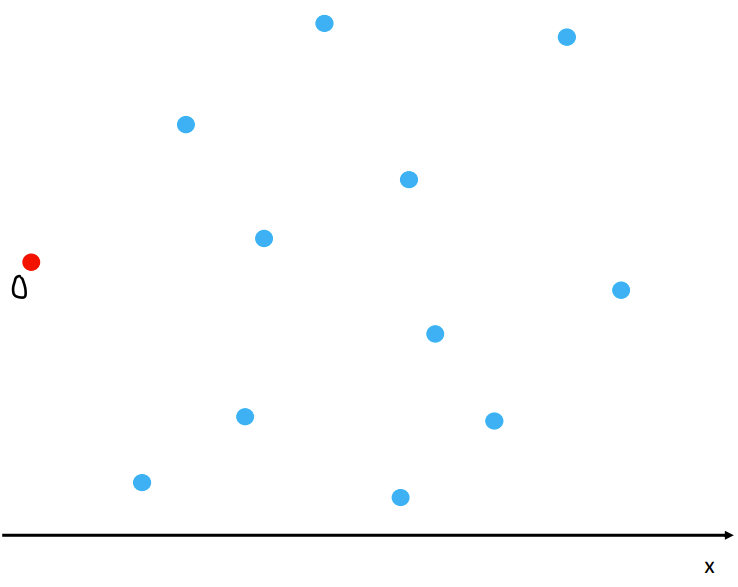
\includegraphics[width=0.3\textwidth]{images/star1.PNG}
        %     \caption{}
        %     \label{fig:star1}
        % \end{figure}

        \begin{figure}[h] 
            \begin{tabular}{ccc}
                \begin{subfigure}{0.33\textwidth}
                    \centering
                    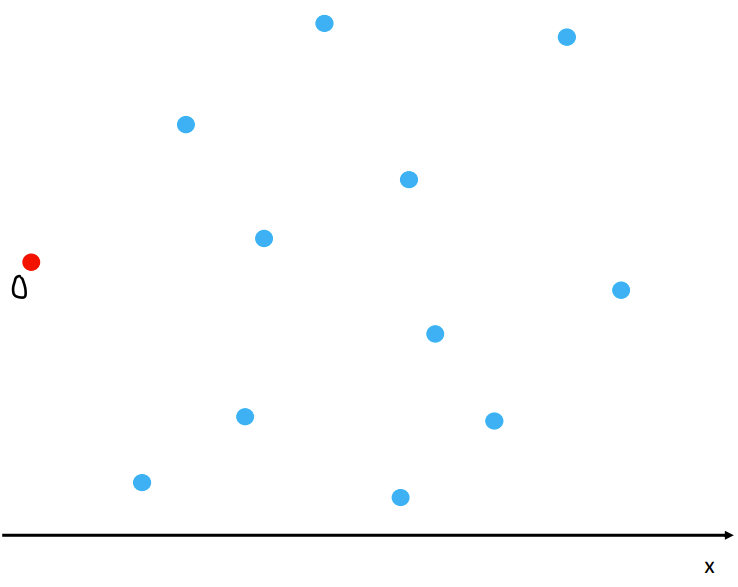
\includegraphics[width=1\textwidth]{images/star1.PNG}
                    \caption{The smallest x-coord point in set $S$ is the leftmost. This point is called $p_0$.}
                    \label{fig:star1}
                \end{subfigure} &
                \begin{subfigure}{0.33\textwidth}
                    \centering
                    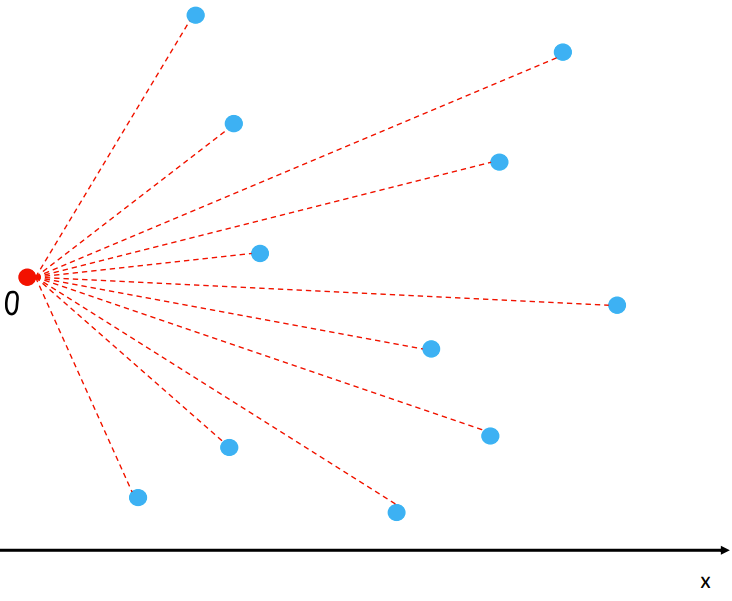
\includegraphics[width=1\textwidth]{images/star2.PNG}
                    \caption{Compute the slope of all line segments from $p_0$ to all other points in $S$.}
                    \label{fig:star2}
                \end{subfigure}&
                \begin{subfigure}{0.33\textwidth}
                    \centering
                    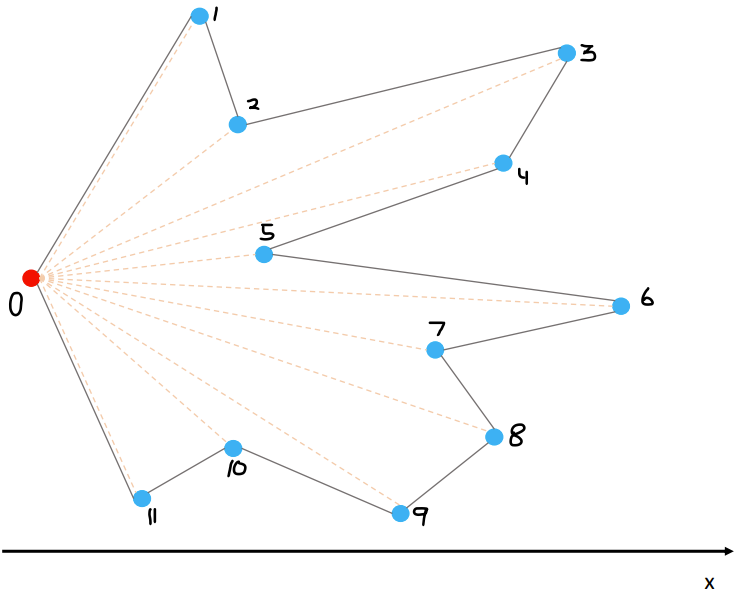
\includegraphics[width=1\textwidth]{images/star3.PNG}
                    \caption{Sorting the vertices by the slope values. $p_0$ is a kernal of star $P$.}
                    \label{fig:star3}
                \end{subfigure} 
            \end{tabular}
            \caption{}
            \label{fig:bigstar}
        \end{figure}

        \pagebreak


        For a set $S$ where $n = 3$ (a triangle), it is trivially a starshaped polygon and the edges of the leftmost vertex ($p_0$) has edges to the other two points. $p_1$ is given by the point that forms the greater slope with $p_0$. $p_2$ is given by the remaining point and is located ``below'' $p_1$ because the slope of $\overline{p_0 p_2}$ is less than the slope of $\overline{p_0 p_1}$, and they do not intersect inside the triangle (Fig. \ref{fig:star4}).

        \begin{figure}[h] 
            \centering
            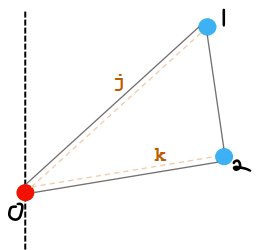
\includegraphics[width=0.3\textwidth]{images/star4.PNG}
            \caption{Slopes are labeled in orange dashed lines. The dashed black line is the vertical line given by the x-coord of $p_0$. Slope $j$ is greater than slope $k$. Vertices then ordered $\{0, 1, 2\}$, and creates a star shape, and all points, not just $p_0$, are kernals.}
            \label{fig:star4}
        \end{figure} 

        

        Let the algorithm hold for set $S$ of size $n$ for the first the $n - 1$ vertices ($\{p_0, ..., p_{n - 2}\} \in P$), such that all the line segments created from $p_0$ to every other point in $P$ is also in $P$. Since the first $n - 1$ vertices of $P$ have already been found, that means they are ordered by their slopes with $p_0$. Then, the $n^{th}$ point of the set $S$ must appear below the last point in $P$ because the slope of $\overline{p_0 p_{n-1}}$ is less than the slope of $\overline{p_0 p_{n - 2}}$. The new edges of polygon $P$ formed by $\overline{p_{n-2} p_{n - 1}}$ and $\overline{p_0 p_{n - 1}}$ replace the previous edge of $\overline{p_0 p_{n - 2}}$. Since $\overline{p_0 p_{n - 1}}$ does not intersect $\overline{p_0 p_{n - 2}}$ execpt at $p_0$, the line segment given by $\overline{p_0 p_{n - 2}}$ still remains inside of polygon $P$ (Fig \ref{fig:normalstar}).

        \begin{figure}[h] 
            \begin{tabular}{cc}
                \begin{subfigure}{0.5\textwidth}
                    \centering
                    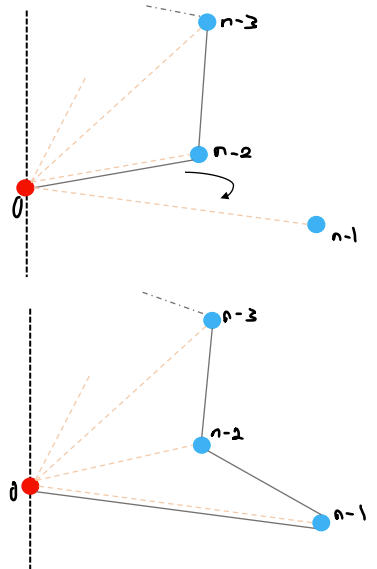
\includegraphics[width=0.7\textwidth]{images/stara.PNG}
                    \caption{A left turn to the next smaller slope point. The kernal still sees all other previous points.}
                    \label{fig:stara}
                \end{subfigure} &
                \begin{subfigure}{0.5\textwidth}
                    \centering
                    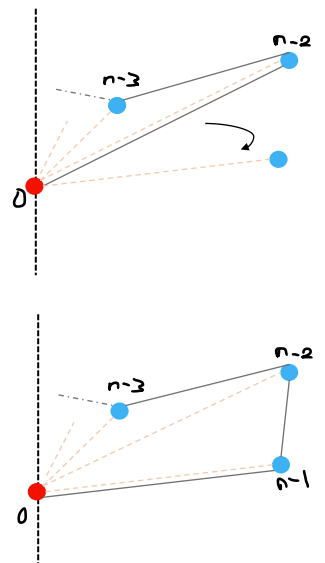
\includegraphics[width=0.6\textwidth]{images/starb.PNG}
                    \caption{a right turn to the next smaller slope point. The kernal still sees all other previous points.}
                    \label{fig:starb}
                \end{subfigure}  
                % \begin{subfigure}{0.5\textwidth}
                %     \centering
                %     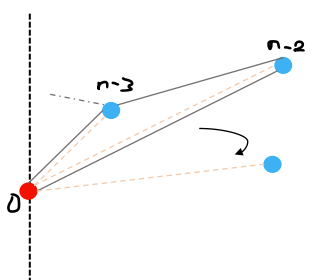
\includegraphics[width=0.7\textwidth]{images/star7.PNG}
                %     \caption{}
                %     \label{fig:star7}
                % \end{subfigure} &
                % \begin{subfigure}{0.5\textwidth}
                %     \centering
                %     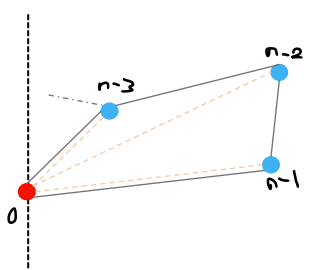
\includegraphics[width=0.7\textwidth]{images/star8.PNG}
                %     \caption{}
                %     \label{fig:star8}
                % \end{subfigure}
                % \begin{subfigure}{0.33\textwidth}
                %     \centering
                %     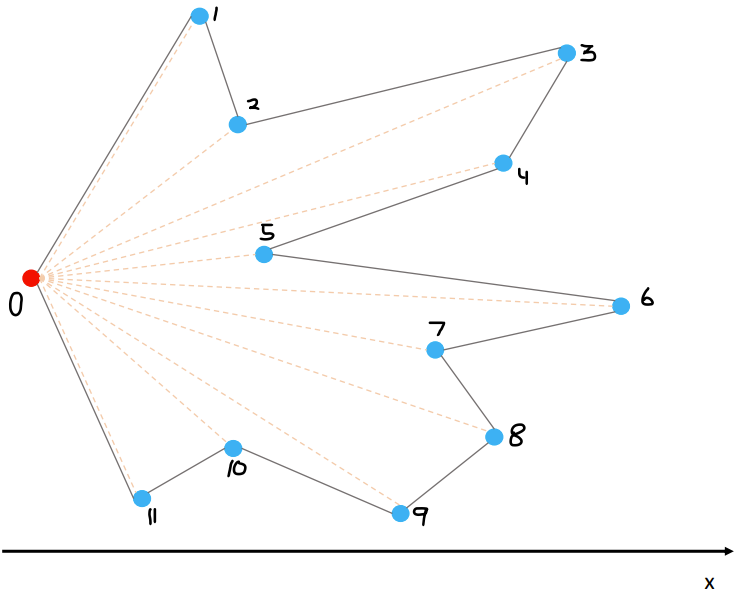
\includegraphics[width=1\textwidth]{images/star3.PNG}
                %     \caption{Sorting the vertices by the slope values. $p_0$ is a kernal of star $P$.}
                %     \label{fig:star3}
                % \end{subfigure} 
            \end{tabular}
            \caption{The turn to the next point doesn't matter if the points are sorted by the slopes from $p_0$. The kernal still sees all previous points if the next point in the set has the next smaller slope.}
            \label{fig:normalstar}
        \end{figure}

        \pagebreak

        The $n^{th}$ point cannot lie ``above'' the $n-1^{th}$ point, because that means the slope of $\overline{p_0 p_{n - 1}}$ was greater than the slope of $\overline{p_0 p_{n - 2}}$. By contradiction, $p_{n-1}$ and $p_{n-2}$ were not in correct sorted order.

        \begin{figure}[h] 
            \centering
            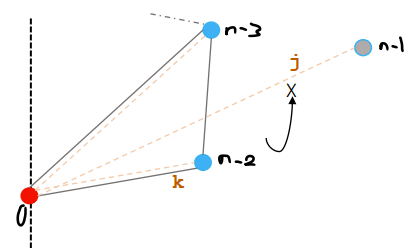
\includegraphics[width=0.4\textwidth]{images/star9.PNG}
            \caption{Slope $j$ is greater than slope $k$. Therefore the above points are out of order.}
            \label{fig:star9}
        \end{figure} 


        \pagebreak

        No points can be ``behind'' $p_0$, i.e. have a smaller x-coord value than $p_0$, because $p_0$ was determined to be the smallest x-coord point in $S$ (Fig. \ref{fig:wrongstar}).

        \begin{figure}[h] 
            \begin{tabular}{cc}
                \begin{subfigure}{0.5\textwidth}
                    \centering
                    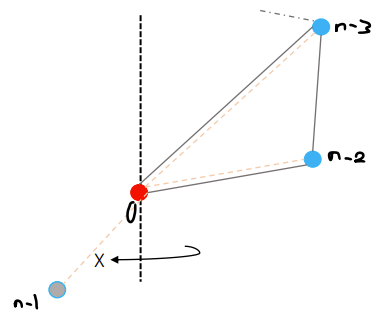
\includegraphics[width=0.8\textwidth]{images/star10.PNG}
                    \caption{The smallest x-coord point in set $S$ is the leftmost. This point is called $p_0$.}
                    \label{fig:star10}
                \end{subfigure} &
                \begin{subfigure}{0.5\textwidth}
                    \centering
                    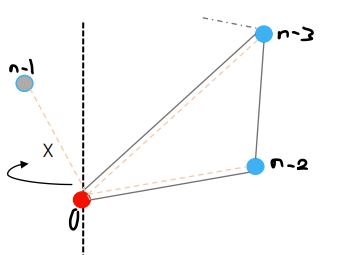
\includegraphics[width=0.7\textwidth]{images/star11.PNG}
                    \caption{Compute the slope of all line segments from $p_0$ to all other points in $S$.}
                    \label{fig:star11}
                \end{subfigure}
            \end{tabular}
            \caption{}
            \label{fig:wrongstar}
        \end{figure}



        \pagebreak
        
        \item For a set of points $Q$ such that $\forall q \in Q$, $q \notin S$, describe algorithms to determine if $q$ is interior or exterior to $P$ and $R$.
        
        \cbcolor{blue}
            \cbstart
            \textsc{RelativeToPolygon($Q$, $N$)}:
            \begin{enumerate}[label=\arabic*.]
                \item 
            \end{enumerate}
        \cbend


        left turn, check above (exterior) or below (interior). 

        right turn, check above (interior) or below (exterior)


        Reference: \cite{officehours}

    \end{enumerate}


    \pagebreak
    % END %%%%%%%%%%%%%%%%%%%%%%%%%%%%%%%%%%%%%%%%%%%%%%%%%%%%%%%%%%%%%%%%%%%



\begin{thebibliography}{1}
\bibitem[1]{crossprod2vec}Cross Product of Two Vectors: \url{https://www.cuemath.com/geometry/cross-product/}
\bibitem[2]{mathcurvorien}Math World - Curve Orientation: \url{https://mathworld.wolfram.com/CurveOrientation.html}
\bibitem[3]{officehours}Jake and Diane's office hours, classmates: Stephanie, Sydney, and MacKenzie with homework problem discussions.
\end{thebibliography}
%%%%%%%%%%%%%%%%%%%%%%%%%%%%%%%%%%%%%%%%%%%%%%%%%%%%%%%%%%%%%%%%%%%%%%
\end{document}
%%%%%%%%%%%%%%%%%%%%%%%%%%%%%%%%%%%%%%%%%%%%%%%%%%%%%%%%%%%%%%%%%%%%%%

